% Made up for the tikra benchmark.
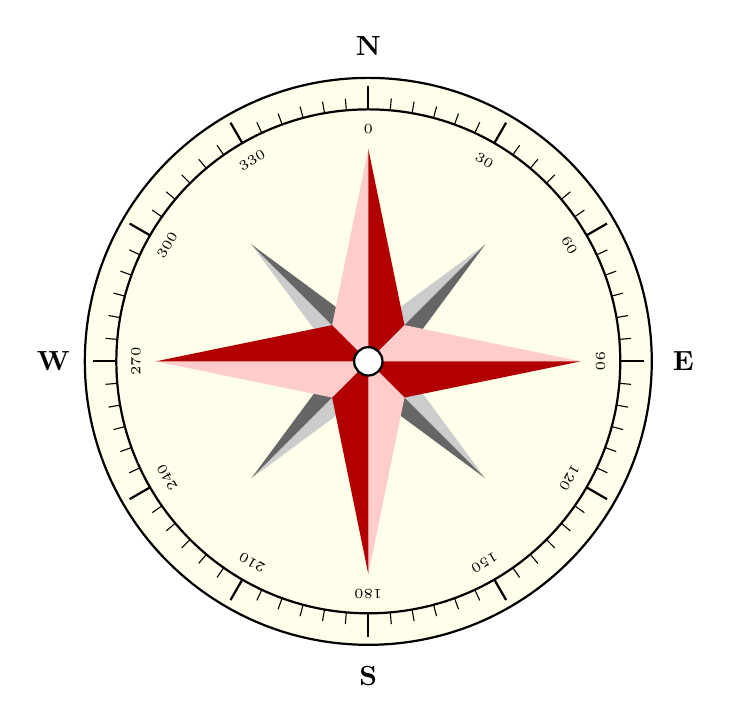
\begin{tikzpicture}[line join=round]
  \fill[yellow!8] (0,0) circle (3.6);
  \draw[thick] (0,0) circle (3.6) circle (3.2);
  \foreach \a in {0,5,...,355} { \draw (\a:3.2) -- (\a:3.35); }
  \foreach \a in {0,30,...,330} {
    \draw[thick] (\a:3.2) -- (\a:3.5);
    \pgfmathtruncatemacro\b{mod(450-\a,360)}
    \node[font=\tiny, rotate=\a-90] at (\a:2.95) {\b};
  }
  % intercardinal points
  \foreach \a in {45,135,225,315} {
    \fill[gray!40] (0,0) -- (\a:2.1) -- (\a+30:0.5) -- cycle;
    \fill[gray!80!black] (0,0) -- (\a:2.1) -- (\a-30:0.5) -- cycle;
  }
  % cardinal points
  \foreach \a/\l in {90/N, 0/E, 270/S, 180/W} {
    \fill[red!20] (0,0) -- (\a:2.7) -- (\a+45:0.65) -- cycle;
    \fill[red!70!black] (0,0) -- (\a:2.7) -- (\a-45:0.65) -- cycle;
  }
  \foreach \a/\l in {90/N, 0/E, 270/S, 180/W} { \node[font=\bfseries] at (\a:4) {\l}; }
  \draw[thick, fill=white] (0,0) circle (0.18);
\end{tikzpicture}
